\section{L'aérostation}

\begin{table}[H]
    \centering
    \begin{tabular}{c l c}
        \begin{minipage}{.075\textwidth}
            \begin{figure}[H]
                \centering
                
\includegraphics[width=1.0\linewidth]{Annexes/friseChronologique/img/Flag_of_France.pdf}
            \end{figure}
        \end{minipage}
    &
        \begin{minipage}{.65\textwidth}
            \textbf{1783} - \textbf{Premier vol en montgolfière}
            
            Pilâtre de Rosier s'élève dans le ciel grâce à la montgolfière des frères Montgoflier
            \begin{figure}[H]
                \legende{Ascension captive d'une montgolfière (Jean-François Pilâtre de Rozier) dans les jardins de la papèterie Réveillon, le 19 octobre 1783.}{frise:Montgolfiere_1783.jpg}
            \end{figure}
        \end{minipage}
    &
        \begin{minipage}{.275\textwidth}
            \begin{figure}[H]
                \centering
                \includegraphics[width=1.0\linewidth]{Annexes/friseChronologique/img/Montgolfiere_1783.jpg}
            \end{figure}
        \end{minipage}
    \end{tabular}
\end{table}
\begin{table}[H]
    \centering
    \begin{tabular}{c l c}
        \begin{minipage}{.075\textwidth}
            \begin{figure}[H]
                \centering
                
\includegraphics[width=1.0\linewidth]{Annexes/friseChronologique/img/Flag_of_France.pdf}
            \end{figure}
        \end{minipage}
    &
        \begin{minipage}{.65\textwidth}
            \textbf{1785} - \textbf{Première traversée de la manche}
            
            Jean-Pierre Blanchard traverse la Manche en ballon
            \begin{figure}[H]
                \legende{Traversée en ballon du Pas-de-Calais par Blanchard et Jefferies (1785)}{frise:Early_flight_02562u_28729.jpg}
            \end{figure}
        \end{minipage}
    &
        \begin{minipage}{.275\textwidth}
            \begin{figure}[H]
                \centering
                \includegraphics[width=1.0\linewidth]{Annexes/friseChronologique/img/Early_flight_02562u_28729.jpg}
            \end{figure}
        \end{minipage}
    \end{tabular}
\end{table}
\begin{table}[H]
    \centering
    \begin{tabular}{c l c}
        \begin{minipage}{.075\textwidth}
            \begin{figure}[H]
                \centering
                
\includegraphics[width=1.0\linewidth]{Annexes/friseChronologique/img/Flag_of_France.pdf}
            \end{figure}
        \end{minipage}
    &
        \begin{minipage}{.65\textwidth}
            \textbf{1797} - \textbf{Premier saut en parachute}
            
            André-Jacques Garnerin effectue le premier saut en parachute, depuis un ballon
            \begin{figure}[H]
                \legende{N°. 4 – Descente de Jacques Garnerin en parachute (1797)}{frise:Early_flight_02561u_28429.jpg}
            \end{figure}
        \end{minipage}
    &
        \begin{minipage}{.275\textwidth}
            \begin{figure}[H]
                \centering
                \includegraphics[width=1.0\linewidth]{Annexes/friseChronologique/img/Early_flight_02561u_28429.jpg}
            \end{figure}
        \end{minipage}
    \end{tabular}
\end{table}
\begin{table}[H]
    \centering
    \begin{tabular}{c l c}
        \begin{minipage}{.075\textwidth}
            \begin{figure}[H]
                \centering
                
\includegraphics[width=1.0\linewidth]{Annexes/friseChronologique/img/Flag_of_France.pdf}
            \end{figure}
        \end{minipage}
    &
        \begin{minipage}{.65\textwidth}
            \textbf{1852} - \textbf{Premier vol en dirigeable}
            
            L'ingénieur français Henri Giffard fit voler le premier dirigeable
        \end{minipage}
    &
        \begin{minipage}{.275\textwidth}
            \begin{figure}[H]
                \centering
                \includegraphics[width=1.0\linewidth]{Annexes/friseChronologique/vide.pdf}
            \end{figure}
        \end{minipage}
    \end{tabular}
\end{table}
\section{Les pionniers du plus lourd que l'air}

\begin{table}[H]
    \centering
    \begin{tabular}{c l c}
        \begin{minipage}{.075\textwidth}
            \begin{figure}[H]
                \centering
                
\includegraphics[width=1.0\linewidth]{Annexes/friseChronologique/img/Flag_of_France.pdf}
            \end{figure}
        \end{minipage}
    &
        \begin{minipage}{.65\textwidth}
            \textbf{1890} - \textbf{Clément Ader met au point l'Eole}
            
            Clément Ader, ingénieur français, conçoit l'Eole puis les Avions, aérodynes en forme de chauves-souris. Bien que Clément Ader affirma à partir de 1906 que ses aérodynes soient parvnus à réaliser des vols de 300 m, on manque de preuve pour attester ces affirmations. Pour cette raison, on ne retient pas Ader comme ayant été le premier à effectuer un vol contrôlé.
        \end{minipage}
    &
        \begin{minipage}{.275\textwidth}
            \begin{figure}[H]
                \centering
                \includegraphics[width=1.0\linewidth]{Annexes/friseChronologique/vide.pdf}
            \end{figure}
        \end{minipage}
    \end{tabular}
\end{table}
\begin{table}[H]
    \centering
    \begin{tabular}{c l c}
        \begin{minipage}{.075\textwidth}
            \begin{figure}[H]
                \centering
                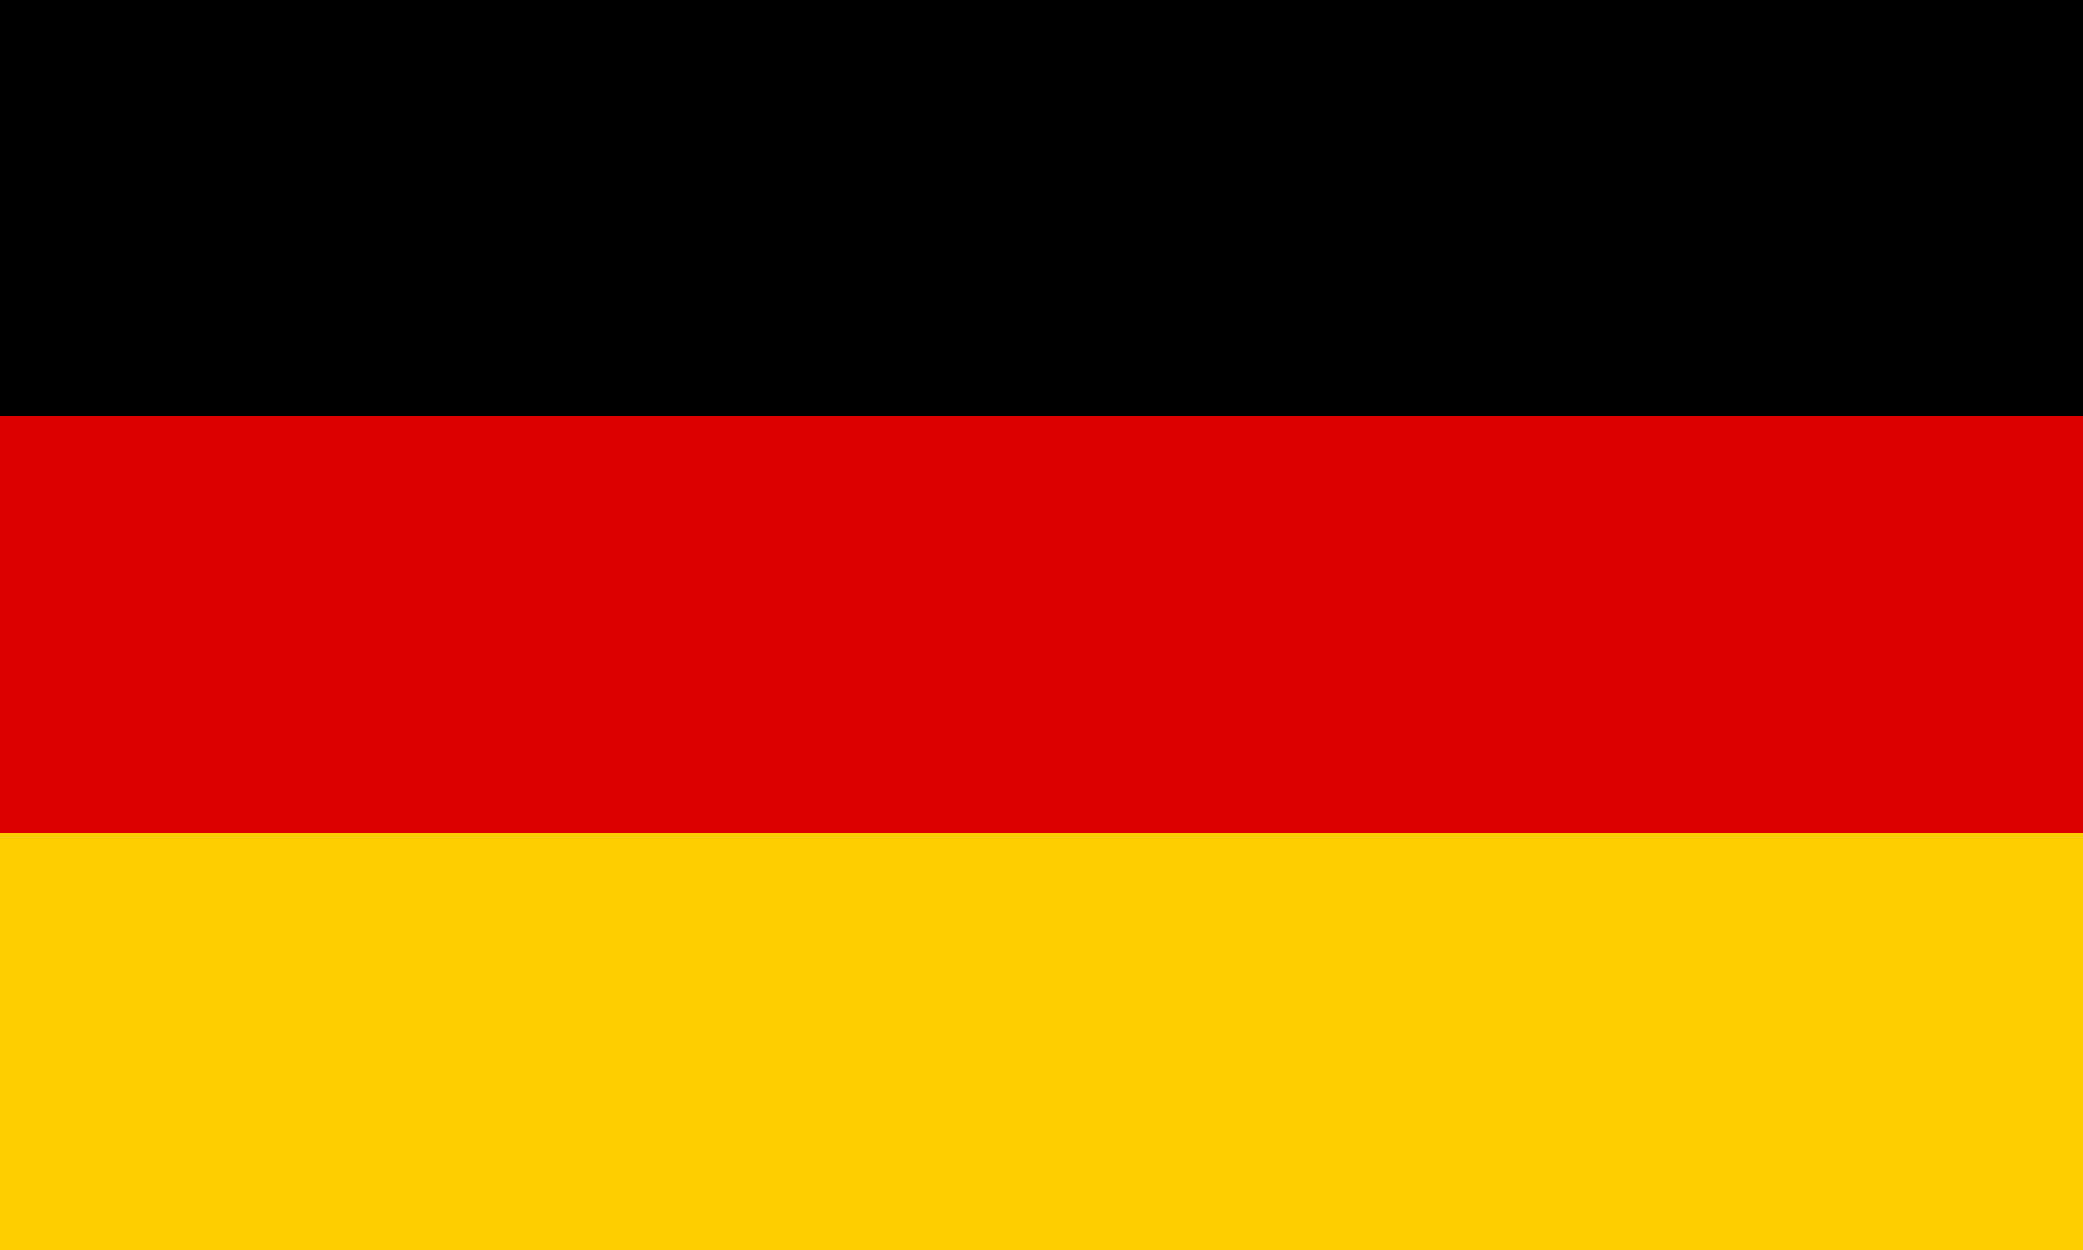
\includegraphics[width=1.0\linewidth]{Annexes/friseChronologique/img/Flag_of_Germany.pdf}
            \end{figure}
        \end{minipage}
    &
        \begin{minipage}{.65\textwidth}
            \textbf{1891} - \textbf{Premier vol en planeur}
            
            L'ingénieur allemand Otto Lilienthal fait voler son planeur, en se lancant depuis une colline
            \begin{figure}[H]
                \legende{L'un des vols d'Otto Lilienthal, ici en 1895}{frise:Otto_Lilienthal_gliding_experiment_ppmsca.02546.jpg}
            \end{figure}
        \end{minipage}
    &
        \begin{minipage}{.275\textwidth}
            \begin{figure}[H]
                \centering
                \includegraphics[width=1.0\linewidth]{Annexes/friseChronologique/img/Otto_Lilienthal_gliding_experiment_ppmsca.02546.jpg}
            \end{figure}
        \end{minipage}
    \end{tabular}
\end{table}
\begin{table}[H]
    \centering
    \begin{tabular}{c l c}
        \begin{minipage}{.075\textwidth}
            \begin{figure}[H]
                \centering
                
\includegraphics[width=1.0\linewidth]{Annexes/friseChronologique/img/Flag_of_France.pdf}
            \end{figure}
        \end{minipage}
    &
        \begin{minipage}{.65\textwidth}
            \textbf{1901} - \textbf{Alberto Santos Dumont contourne la Tour Eiffel en dirigeable}
            
            
            \begin{figure}[H]
                \legende{Internet Archive Book Images}{frise:Santos-Dumont_flight_around_the_Eiffel_Tower.jpg}
            \end{figure}
        \end{minipage}
    &
        \begin{minipage}{.275\textwidth}
            \begin{figure}[H]
                \centering
                \includegraphics[width=1.0\linewidth]{Annexes/friseChronologique/img/Santos-Dumont_flight_around_the_Eiffel_Tower.jpg}
            \end{figure}
        \end{minipage}
    \end{tabular}
\end{table}
\begin{table}[H]
    \centering
    \begin{tabular}{c l c}
        \begin{minipage}{.075\textwidth}
            \begin{figure}[H]
                \centering
                
\includegraphics[width=1.0\linewidth]{Annexes/friseChronologique/img/Flag_of_the_United_States_28DDD-F-416E_specifications29.pdf}
            \end{figure}
        \end{minipage}
    &
        \begin{minipage}{.65\textwidth}
            \textbf{1903} - \textbf{Premier vol d'un avion}
            
            Les frères Orville et Wilbur Wright font voler leur avion aux Etats-Unis.
Il s'agit du premier vol contrôlé d'un aérodyne motorisé
            \begin{figure}[H]
                \legende{Premier vol motorisé des frères Wright le 17 décembre 1903 sur Flyer.}{frise:Wrightflyer.jpg}
            \end{figure}
        \end{minipage}
    &
        \begin{minipage}{.275\textwidth}
            \begin{figure}[H]
                \centering
                \includegraphics[width=1.0\linewidth]{Annexes/friseChronologique/img/Wrightflyer.jpg}
            \end{figure}
        \end{minipage}
    \end{tabular}
\end{table}
\begin{table}[H]
    \centering
    \begin{tabular}{c l c}
        \begin{minipage}{.075\textwidth}
            \begin{figure}[H]
                \centering
                
\includegraphics[width=1.0\linewidth]{Annexes/friseChronologique/img/Flag_of_France.pdf}
            \end{figure}
        \end{minipage}
    &
        \begin{minipage}{.65\textwidth}
            \textbf{1909} - \textbf{Louis Blériot traverse la manche}
            
            "L'Angleterre n'est plus une île !" Le 25 juillet 1909, Louis Blériot relie Calais à Douvres à bord de son  Blériot XI.
            \begin{figure}[H]
                \legende{Blériot aux commandes de l'appareil de la traversée à la fête de Port-Aviation, le 4 juillet 1909.}{frise:Btv1b8433368f-p044_BlC3A9riot_C3A0_la_fC3AAte_de_Port-Aviation2C_dimanche_4_juillet_1909.jpg}
            \end{figure}
        \end{minipage}
    &
        \begin{minipage}{.275\textwidth}
            \begin{figure}[H]
                \centering
                \includegraphics[width=1.0\linewidth]{Annexes/friseChronologique/img/Btv1b8433368f-p044_BlC3A9riot_C3A0_la_fC3AAte_de_Port-Aviation2C_dimanche_4_juillet_1909.jpg}
            \end{figure}
        \end{minipage}
    \end{tabular}
\end{table}
\begin{table}[H]
    \centering
    \begin{tabular}{c l c}
        \begin{minipage}{.075\textwidth}
            \begin{figure}[H]
                \centering
                
\includegraphics[width=1.0\linewidth]{Annexes/friseChronologique/img/Flag_of_France.pdf}
            \end{figure}
        \end{minipage}
    &
        \begin{minipage}{.65\textwidth}
            \textbf{1910} - \textbf{Élisa Deroche, première femme brevetée pilote}
            
            Élisa Deroche s'interesse à l'aviation depuis l'année 1906.
Fin 1909, elle effectue son premier vol solo, et son brevet lui sera délivré quelques mois plus tard, le 8 mars 1910.

La semaine internationale des femmes de l'air marque désormais chaque année cette date historique, puisque cette semaine est positionnée sur la semaine du 8 mars. 

            \begin{figure}[H]
                \legende{Elise Deroche aux commandes d'un biplan Voisin.}{frise:Les_Maitres_de_l27aviation._Mme._la_Baronne_de_Laroche2C_aviatrice2C_au_poste_de_direction_d27un_biplan_Voisin._cph.3c07402.jpg}
            \end{figure}
        \end{minipage}
    &
        \begin{minipage}{.275\textwidth}
            \begin{figure}[H]
                \centering
                \includegraphics[width=1.0\linewidth]{Annexes/friseChronologique/img/Les_Maitres_de_l27aviation._Mme._la_Baronne_de_Laroche2C_aviatrice2C_au_poste_de_direction_d27un_biplan_Voisin._cph.3c07402.jpg}
            \end{figure}
        \end{minipage}
    \end{tabular}
\end{table}
\begin{table}[H]
    \centering
    \begin{tabular}{c l c}
        \begin{minipage}{.075\textwidth}
            \begin{figure}[H]
                \centering
                
\includegraphics[width=1.0\linewidth]{Annexes/friseChronologique/img/Flag_of_France.pdf}
            \end{figure}
        \end{minipage}
    &
        \begin{minipage}{.65\textwidth}
            \textbf{1910} - \textbf{Premier vol d'un hydravion}
            
            L'ingénieur français Henri Fabre devient le premier à décoller d'un plan d'eau avec un aéronef qui dispose de son propre moyen de propulsion. Cette date marque l'entrée dans l'ère de l'hydraviation qui aura son âge d'or sur la période de l'entre 2 guerres.
        \end{minipage}
    &
        \begin{minipage}{.275\textwidth}
            \begin{figure}[H]
                \centering
                \includegraphics[width=1.0\linewidth]{Annexes/friseChronologique/vide.pdf}
            \end{figure}
        \end{minipage}
    \end{tabular}
\end{table}
\begin{table}[H]
    \centering
    \begin{tabular}{c l c}
        \begin{minipage}{.075\textwidth}
            \begin{figure}[H]
                \centering
                
\includegraphics[width=1.0\linewidth]{Annexes/friseChronologique/img/Flag_of_France.pdf}
            \end{figure}
        \end{minipage}
    &
        \begin{minipage}{.65\textwidth}
            \textbf{1913} - \textbf{Adolphe Pégoud : premier looping}
            
            
        \end{minipage}
    &
        \begin{minipage}{.275\textwidth}
            \begin{figure}[H]
                \centering
                \includegraphics[width=1.0\linewidth]{Annexes/friseChronologique/vide.pdf}
            \end{figure}
        \end{minipage}
    \end{tabular}
\end{table}
\section{La première guerre mondiale}

\begin{table}[H]
    \centering
    \begin{tabular}{c l c}
        \begin{minipage}{.075\textwidth}
            \begin{figure}[H]
                \centering
                
\includegraphics[width=1.0\linewidth]{Annexes/friseChronologique/img/Flag_of_France.pdf}
            \end{figure}
        \end{minipage}
    &
        \begin{minipage}{.65\textwidth}
            \textbf{1914} - \textbf{René Fonck, as des as}
            
            René Fonck est le pilote français ayant le plus grand nombre de victoires aériennes (75). Il est surnomé "l'as des as"
        \end{minipage}
    &
        \begin{minipage}{.275\textwidth}
            \begin{figure}[H]
                \centering
                \includegraphics[width=1.0\linewidth]{Annexes/friseChronologique/vide.pdf}
            \end{figure}
        \end{minipage}
    \end{tabular}
\end{table}
\begin{table}[H]
    \centering
    \begin{tabular}{c l c}
        \begin{minipage}{.075\textwidth}
            \begin{figure}[H]
                \centering
                
\includegraphics[width=1.0\linewidth]{Annexes/friseChronologique/img/Flag_of_Germany_281867E28093191829.pdf}
            \end{figure}
        \end{minipage}
    &
        \begin{minipage}{.65\textwidth}
            \textbf{1914} - \textbf{Manfred von Richtoffen, as de la première guerre mondiale}
            
            Manfred von Richtoffen, pilote allemand, dispose du plus grand nombre de victoires confirmées (80) lors du premier conflit mondial
        \end{minipage}
    &
        \begin{minipage}{.275\textwidth}
            \begin{figure}[H]
                \centering
                \includegraphics[width=1.0\linewidth]{Annexes/friseChronologique/vide.pdf}
            \end{figure}
        \end{minipage}
    \end{tabular}
\end{table}
\section{L'entre 2 guerres}

\begin{table}[H]
    \centering
    \begin{tabular}{c l c}
        \begin{minipage}{.075\textwidth}
            \begin{figure}[H]
                \centering
                
\includegraphics[width=1.0\linewidth]{Annexes/friseChronologique/img/Flag_of_France.pdf}
            \end{figure}
        \end{minipage}
    &
        \begin{minipage}{.65\textwidth}
            \textbf{1918} - \textbf{Georges Latécoère lance l'Aéropostale}
            
            L'Aéropostale est le transport de courrier et frets (colis) par voie aérienne.

Le 25 décembre 1918, il ouvre la ligne entre Toulouse et Barcelone.

Dès 1919, la ligne est étendue jusqu'à Casablanca. Elle sera par la suite prolongée jusqu'à Dakar puis l'amérique du Sud via Rio au Brésil, puis jusqu'à Buenos-Aires et Santiago du Chili
        \end{minipage}
    &
        \begin{minipage}{.275\textwidth}
            \begin{figure}[H]
                \centering
                \includegraphics[width=1.0\linewidth]{Annexes/friseChronologique/vide.pdf}
            \end{figure}
        \end{minipage}
    \end{tabular}
\end{table}
\begin{table}[H]
    \centering
    \begin{tabular}{c l c}
        \begin{minipage}{.075\textwidth}
            \begin{figure}[H]
                \centering
                
\includegraphics[width=1.0\linewidth]{Annexes/friseChronologique/img/Flag_of_France.pdf}
            \end{figure}
        \end{minipage}
    &
        \begin{minipage}{.65\textwidth}
            \textbf{1921} - \textbf{Adrienne Bolland, première femme à traverser la Cordillière des Andes}
            
            Adrienne Bolland traverse la Cordillière en Caudron G3 en 4h15
            \begin{figure}[H]
                \legende{Adrienne Bolland faisant la couverture du magazine argentin El Gráfico le 19 mars 1921}{frise:Adrienne_Bolland_-_El_GrC3A1fico_91.jpg}
            \end{figure}
        \end{minipage}
    &
        \begin{minipage}{.275\textwidth}
            \begin{figure}[H]
                \centering
                \includegraphics[width=1.0\linewidth]{Annexes/friseChronologique/img/Adrienne_Bolland_-_El_GrC3A1fico_91.jpg}
            \end{figure}
        \end{minipage}
    \end{tabular}
\end{table}
\begin{table}[H]
    \centering
    \begin{tabular}{c l c}
        \begin{minipage}{.075\textwidth}
            \begin{figure}[H]
                \centering
                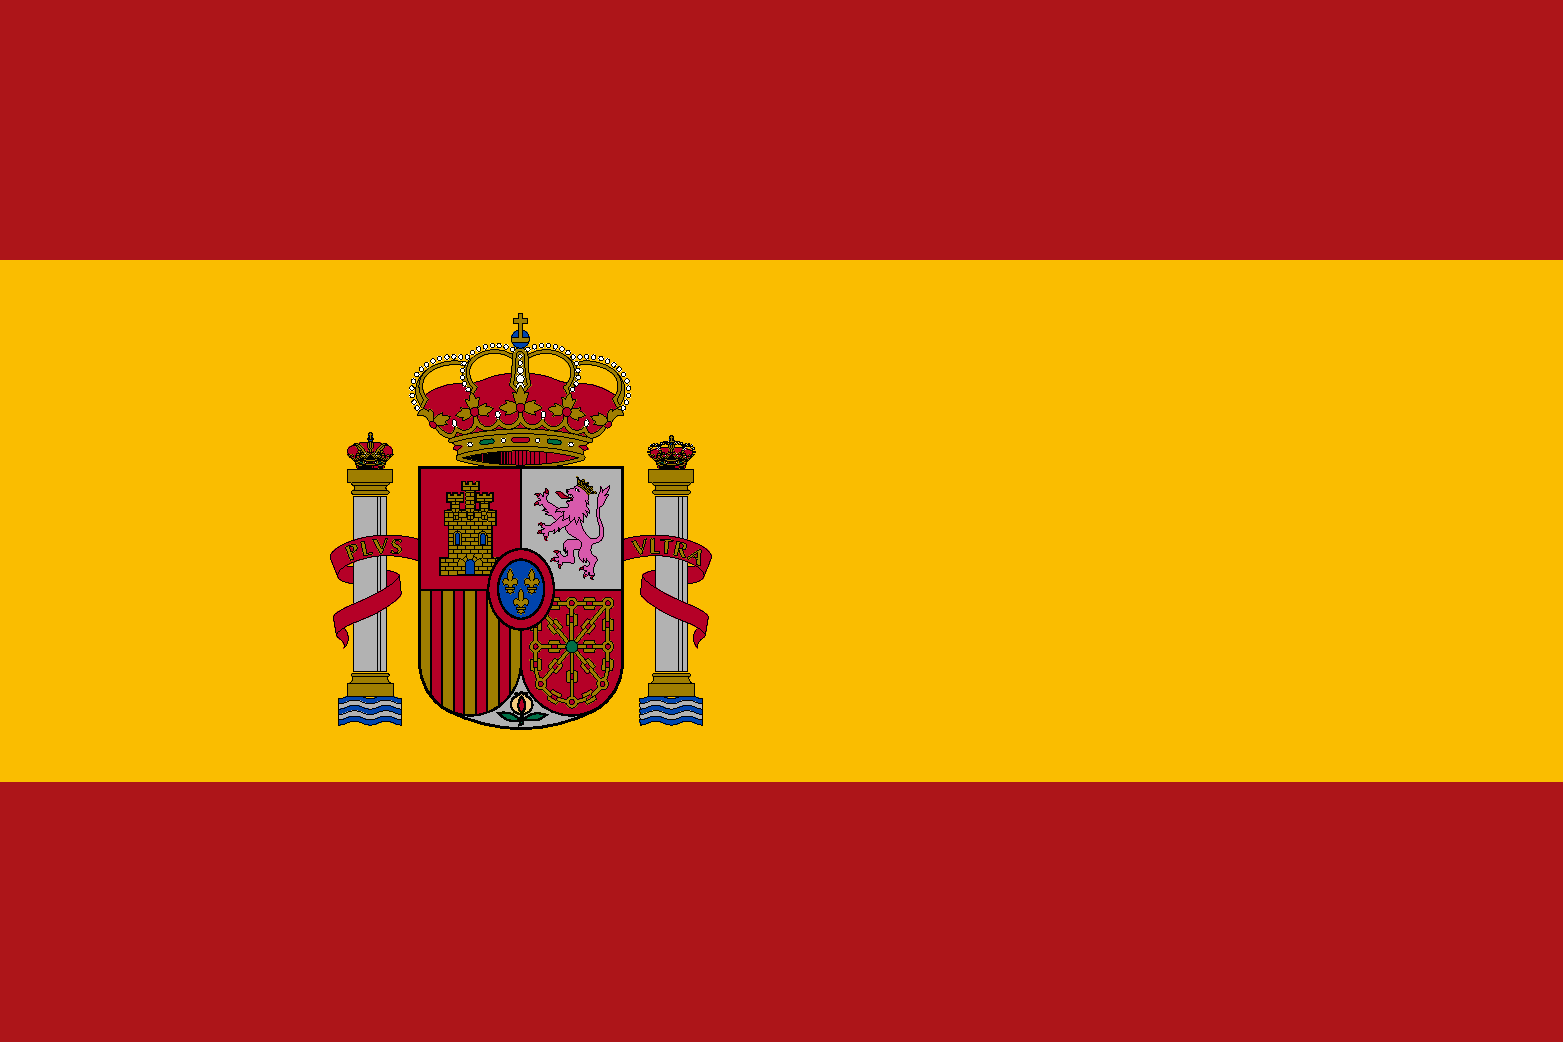
\includegraphics[width=1.0\linewidth]{Annexes/friseChronologique/img/Flag_of_Spain.pdf}
            \end{figure}
        \end{minipage}
    &
        \begin{minipage}{.65\textwidth}
            \textbf{1923} - \textbf{Premier vol d'un autogire}
            
            Juan de la Cierva effectue le premier vol d'un autogire
            \begin{figure}[H]
                \legende{L'autogire C-6 de Juan de la Cierva (1925)}{frise:Autogyro_at_Farnborough2C_1925_28Our_Generation2C_193829.jpg}
            \end{figure}
        \end{minipage}
    &
        \begin{minipage}{.275\textwidth}
            \begin{figure}[H]
                \centering
                \includegraphics[width=1.0\linewidth]{Annexes/friseChronologique/img/Autogyro_at_Farnborough2C_1925_28Our_Generation2C_193829.jpg}
            \end{figure}
        \end{minipage}
    \end{tabular}
\end{table}
\begin{table}[H]
    \centering
    \begin{tabular}{c l c}
        \begin{minipage}{.075\textwidth}
            \begin{figure}[H]
                \centering
                
\includegraphics[width=1.0\linewidth]{Annexes/friseChronologique/img/Flag_of_the_United_States_28DDD-F-416E_specifications29.pdf}
            \end{figure}
        \end{minipage}
    &
        \begin{minipage}{.65\textwidth}
            \textbf{1927} - \textbf{Charles Lindbergh réalise le premier vol transaltantique }
            
            Charles Lindbergh réalise le premier vol transaltantique entre New-York et Paris, à bord de son avion,  le Spirit of Saint-Louis
            \begin{figure}[H]
                \legende{}{frise:Col_Charles_Lindbergh2C_original2C_hec.21329.jpg}
            \end{figure}
        \end{minipage}
    &
        \begin{minipage}{.275\textwidth}
            \begin{figure}[H]
                \centering
                \includegraphics[width=1.0\linewidth]{Annexes/friseChronologique/img/Col_Charles_Lindbergh2C_original2C_hec.21329.jpg}
            \end{figure}
        \end{minipage}
    \end{tabular}
\end{table}
\begin{table}[H]
    \centering
    \begin{tabular}{c l c}
        \begin{minipage}{.075\textwidth}
            \begin{figure}[H]
                \centering
                
\includegraphics[width=1.0\linewidth]{Annexes/friseChronologique/img/Flag_of_France.pdf}
            \end{figure}
        \end{minipage}
    &
        \begin{minipage}{.65\textwidth}
            \textbf{1928} - \textbf{Maryse Bastié, première recordwomen de distance}
            
            
        \end{minipage}
    &
        \begin{minipage}{.275\textwidth}
            \begin{figure}[H]
                \centering
                \includegraphics[width=1.0\linewidth]{Annexes/friseChronologique/vide.pdf}
            \end{figure}
        \end{minipage}
    \end{tabular}
\end{table}
\begin{table}[H]
    \centering
    \begin{tabular}{c l c}
        \begin{minipage}{.075\textwidth}
            \begin{figure}[H]
                \centering
                
\includegraphics[width=1.0\linewidth]{Annexes/friseChronologique/img/Flag_of_the_United_States_28DDD-F-416E_specifications29.pdf}
            \end{figure}
        \end{minipage}
    &
        \begin{minipage}{.65\textwidth}
            \textbf{1932} - \textbf{Amelia Earhart traverse l'Atlantique en solitaire}
            
            En 1928, Amelia Earhart traverse l'Atlantique avec Wilmer Stultz et Louis Gordon. Elle devient ainsi la première femme à effectuer une transatlantique en avion.

Le 20 mai 1932, elle réitere la traversée, mais cette fois ci, seule. Elle effectue en une quinzaine d'heures sur son Lockheed Vega la traversée entre entre le Canada et l'Irlande du Nord.
            \begin{figure}[H]
                \legende{Amelia Earhart en 1935}{frise:Amelia_Earhart_1935.jpg}
            \end{figure}
        \end{minipage}
    &
        \begin{minipage}{.275\textwidth}
            \begin{figure}[H]
                \centering
                \includegraphics[width=1.0\linewidth]{Annexes/friseChronologique/img/Amelia_Earhart_1935.jpg}
            \end{figure}
        \end{minipage}
    \end{tabular}
\end{table}
\begin{table}[H]
    \centering
    \begin{tabular}{c l c}
        \begin{minipage}{.075\textwidth}
            \begin{figure}[H]
                \centering
                
\includegraphics[width=1.0\linewidth]{Annexes/friseChronologique/img/Flag_of_France.pdf}
            \end{figure}
        \end{minipage}
    &
        \begin{minipage}{.65\textwidth}
            \textbf{1933} - \textbf{Création de la compagnie AIr France}
            
            
            \begin{figure}[H]
                \legende{Un Lockheed Super Constellation d'Air France à Heathrow en 1955}{frise:Lockheed_L1049_F-BGNG_Air_France_LAP_08.04.55_edited-2.jpg}
            \end{figure}
        \end{minipage}
    &
        \begin{minipage}{.275\textwidth}
            \begin{figure}[H]
                \centering
                \includegraphics[width=1.0\linewidth]{Annexes/friseChronologique/img/Lockheed_L1049_F-BGNG_Air_France_LAP_08.04.55_edited-2.jpg}
            \end{figure}
        \end{minipage}
    \end{tabular}
\end{table}
\begin{table}[H]
    \centering
    \begin{tabular}{c l c}
        \begin{minipage}{.075\textwidth}
            \begin{figure}[H]
                \centering
                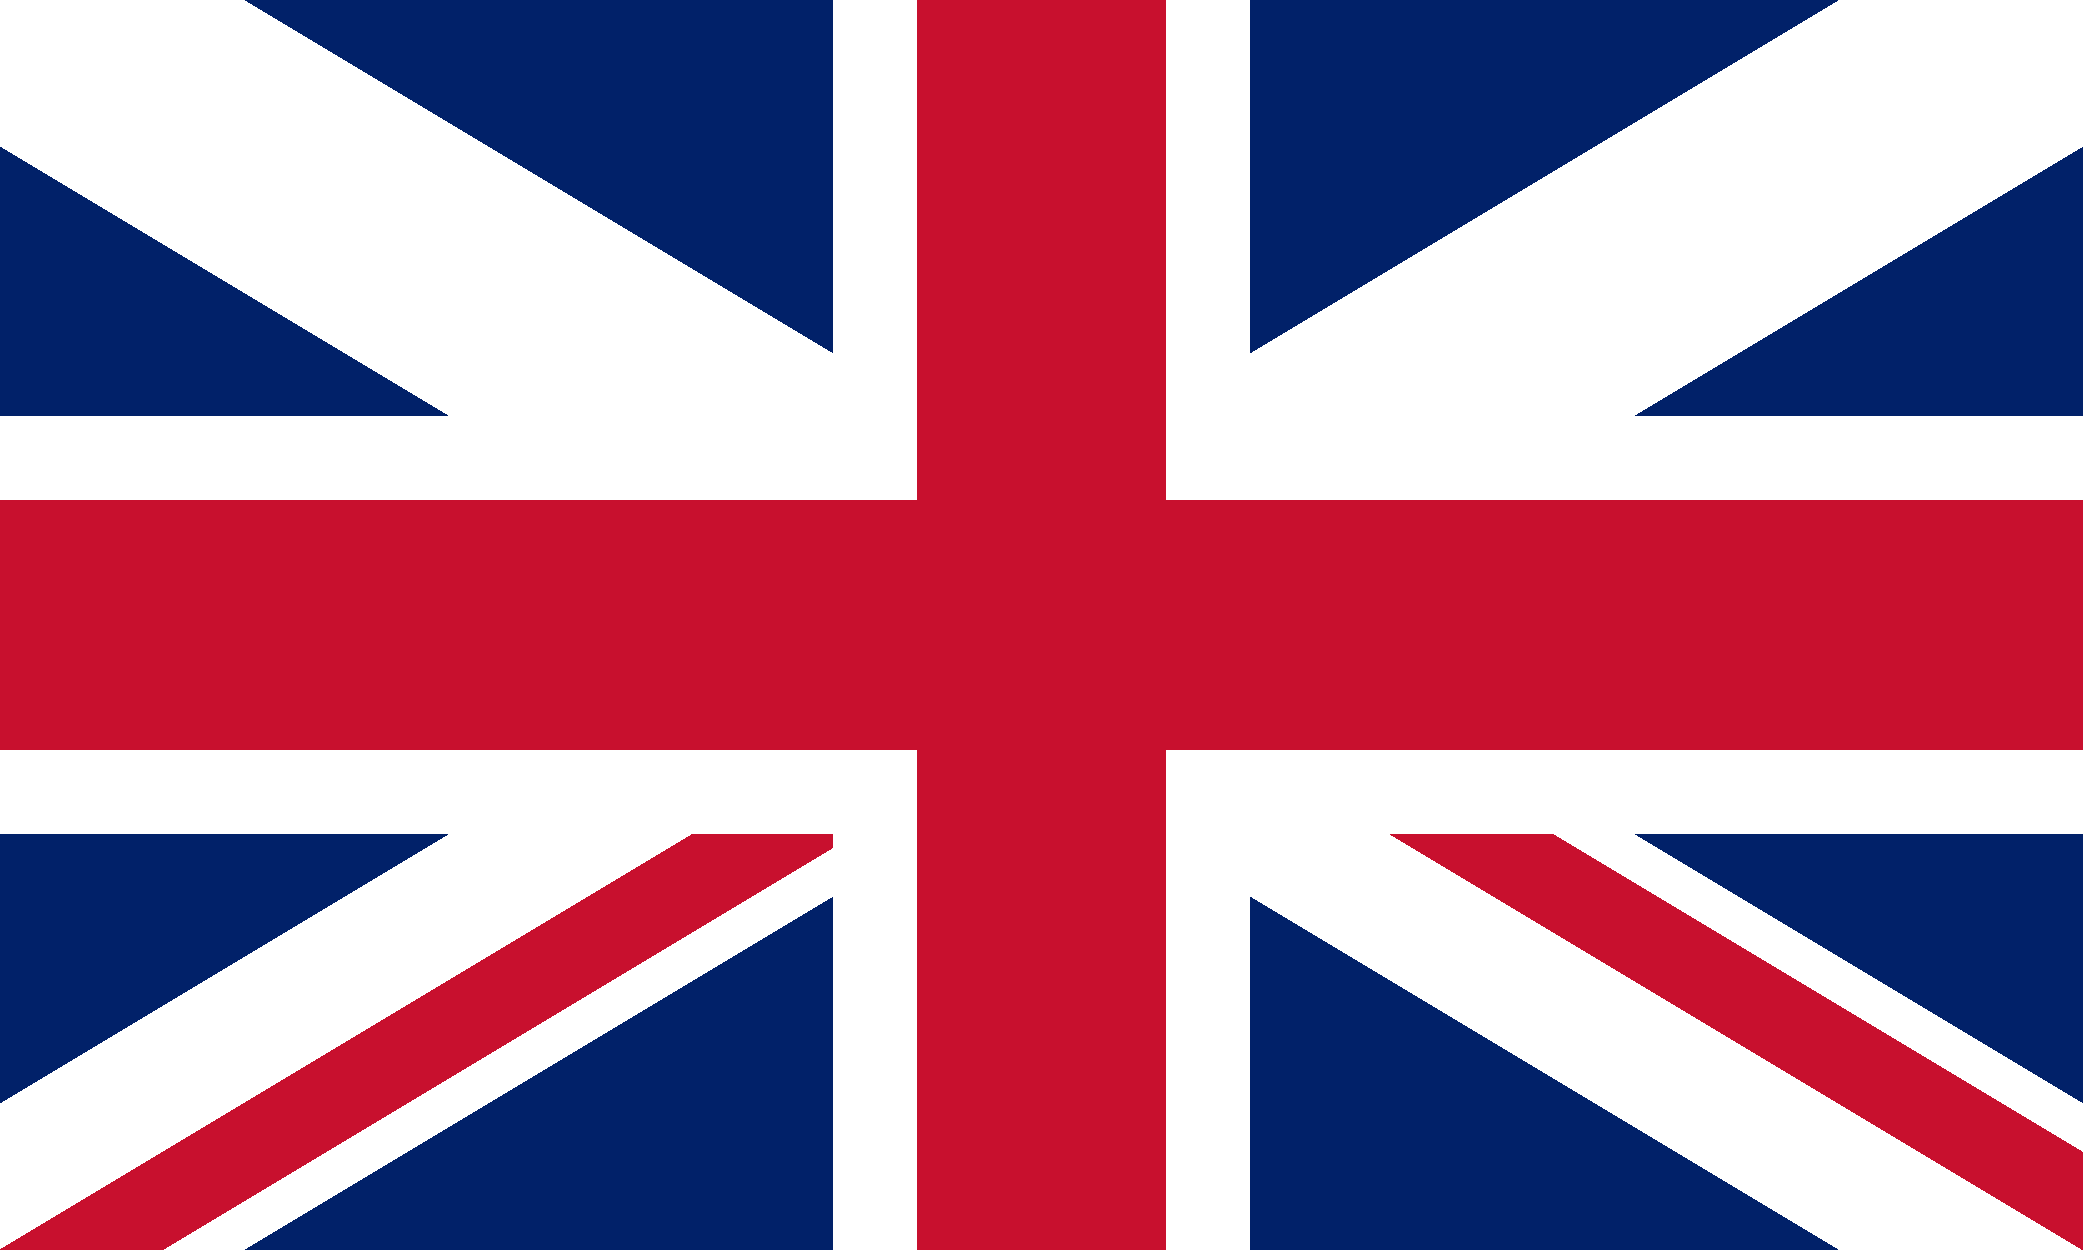
\includegraphics[width=1.0\linewidth]{Annexes/friseChronologique/img/Flag_of_the_United_Kingdom_283-529.pdf}
            \end{figure}
        \end{minipage}
    &
        \begin{minipage}{.65\textwidth}
            \textbf{1935} - \textbf{Robert Watson-Watt invente le radar}
            
            Le britannique Robert Watson-Watt dépose un brevet pour le radar, qui permet de détecter à distance des objets, et notamment des avions. Durant la seconde guerre mondiale, cett invention donnera un avantage décisif aux britanniques durant la bataille d'Angleterre (1940)
            \begin{figure}[H]
                \legende{Composant d'un radar conçu par Robet Watson-Watt}{frise:Watson_Radar.jpg}
            \end{figure}
        \end{minipage}
    &
        \begin{minipage}{.275\textwidth}
            \begin{figure}[H]
                \centering
                \includegraphics[width=1.0\linewidth]{Annexes/friseChronologique/img/Watson_Radar.jpg}
            \end{figure}
        \end{minipage}
    \end{tabular}
\end{table}
\begin{table}[H]
    \centering
    \begin{tabular}{c l c}
        \begin{minipage}{.075\textwidth}
            \begin{figure}[H]
                \centering
                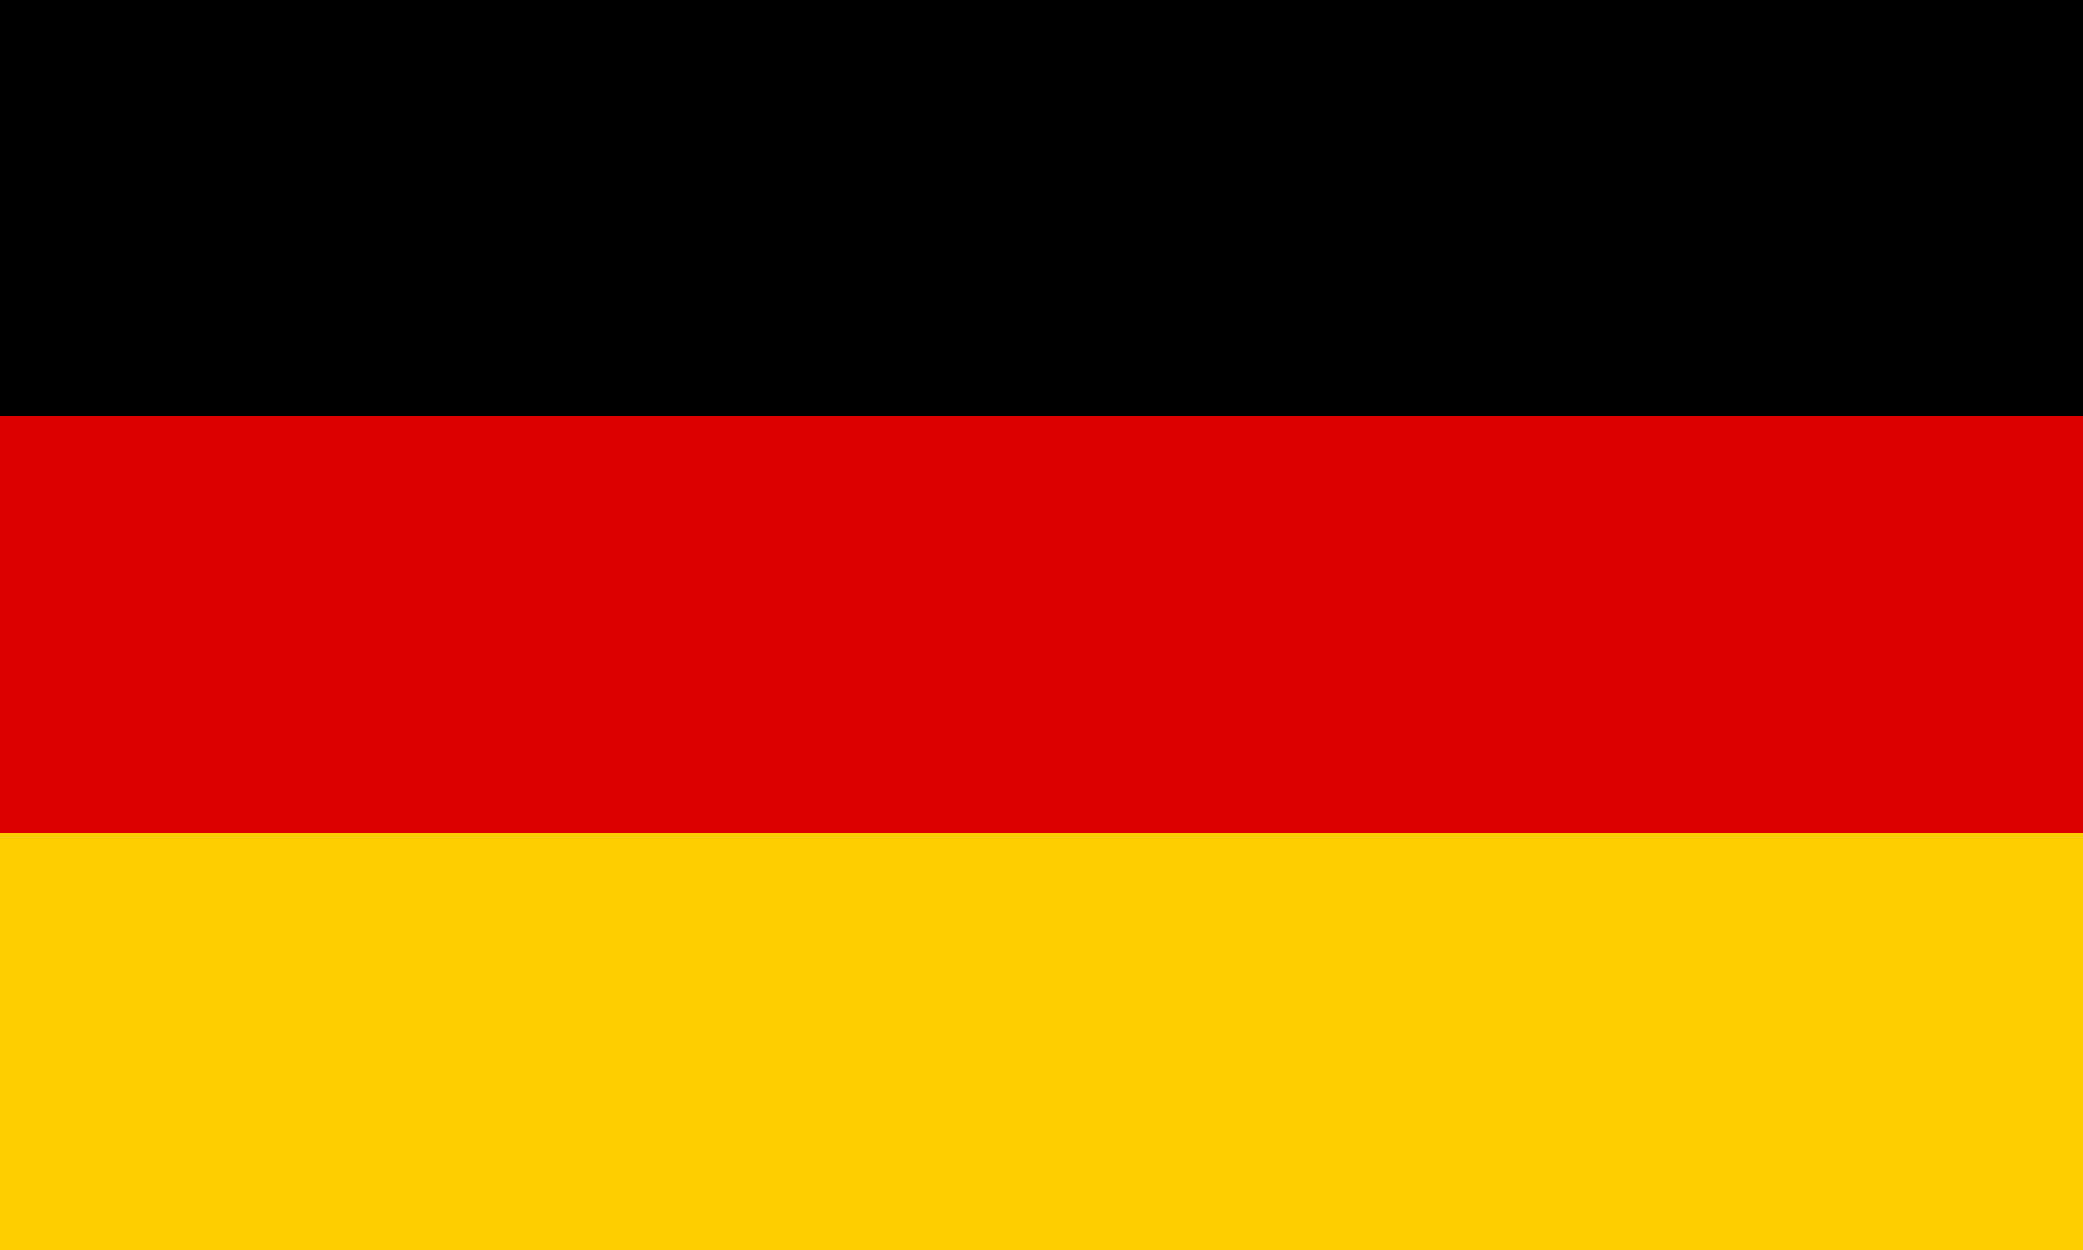
\includegraphics[width=1.0\linewidth]{Annexes/friseChronologique/img/Flag_of_Germany.pdf}
            \end{figure}
        \end{minipage}
    &
        \begin{minipage}{.65\textwidth}
            \textbf{1936} - \textbf{Premier vol d'un hélicoptère}
            
            Le Focke-Wulf Fw 61 est le premier hélicoptère ayant effecuté un vol totalement contrôlé
            \begin{figure}[H]
                \legende{Le Focke-Wulf Fw 61 en vol}{frise:Fw_61_V.JPG}
            \end{figure}
        \end{minipage}
    &
        \begin{minipage}{.275\textwidth}
            \begin{figure}[H]
                \centering
                \includegraphics[width=1.0\linewidth]{Annexes/friseChronologique/img/Fw_61_V.JPG}
            \end{figure}
        \end{minipage}
    \end{tabular}
\end{table}
\begin{table}[H]
    \centering
    \begin{tabular}{c l c}
        \begin{minipage}{.075\textwidth}
            \begin{figure}[H]
                \centering
                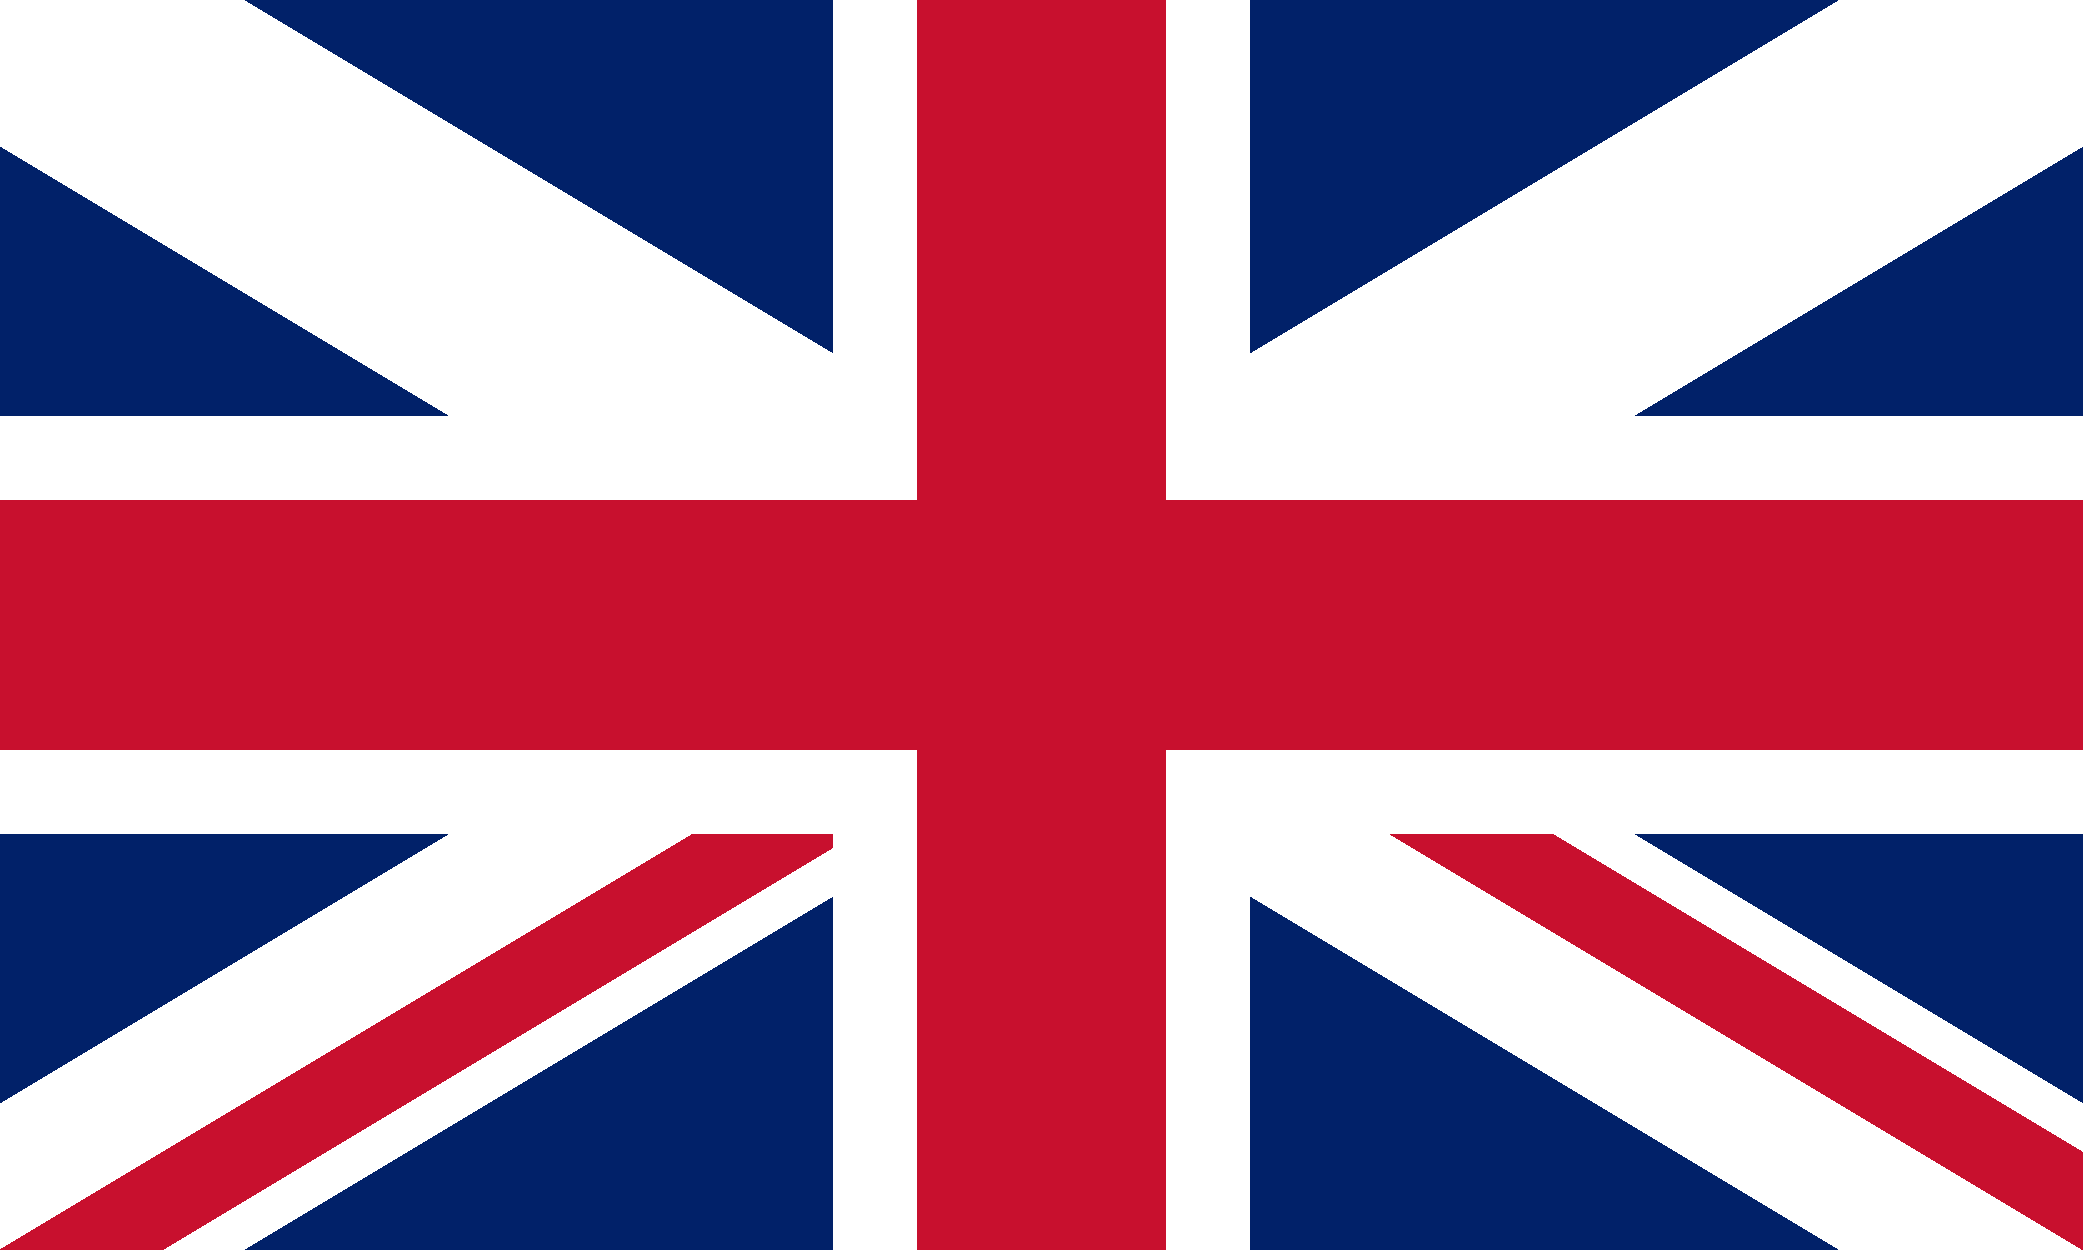
\includegraphics[width=1.0\linewidth]{Annexes/friseChronologique/img/Flag_of_the_United_Kingdom_283-529.pdf}
            \end{figure}
        \end{minipage}
    &
        \begin{minipage}{.65\textwidth}
            \textbf{1936} - \textbf{Premier vol du Spitfire}
            
            Le Supermarine Spitfire est un chasseur à hélice. Il sera considéré comme le meilleur avion de la seconde guerre mondiale.
            \begin{figure}[H]
                \legende{Un Spitfire}{frise:Ray_Flying_Legends_2005-1.jpg}
            \end{figure}
        \end{minipage}
    &
        \begin{minipage}{.275\textwidth}
            \begin{figure}[H]
                \centering
                \includegraphics[width=1.0\linewidth]{Annexes/friseChronologique/img/Ray_Flying_Legends_2005-1.jpg}
            \end{figure}
        \end{minipage}
    \end{tabular}
\end{table}
\section{La seconde guerre mondiale}

\begin{table}[H]
    \centering
    \begin{tabular}{c l c}
        \begin{minipage}{.075\textwidth}
            \begin{figure}[H]
                \centering
                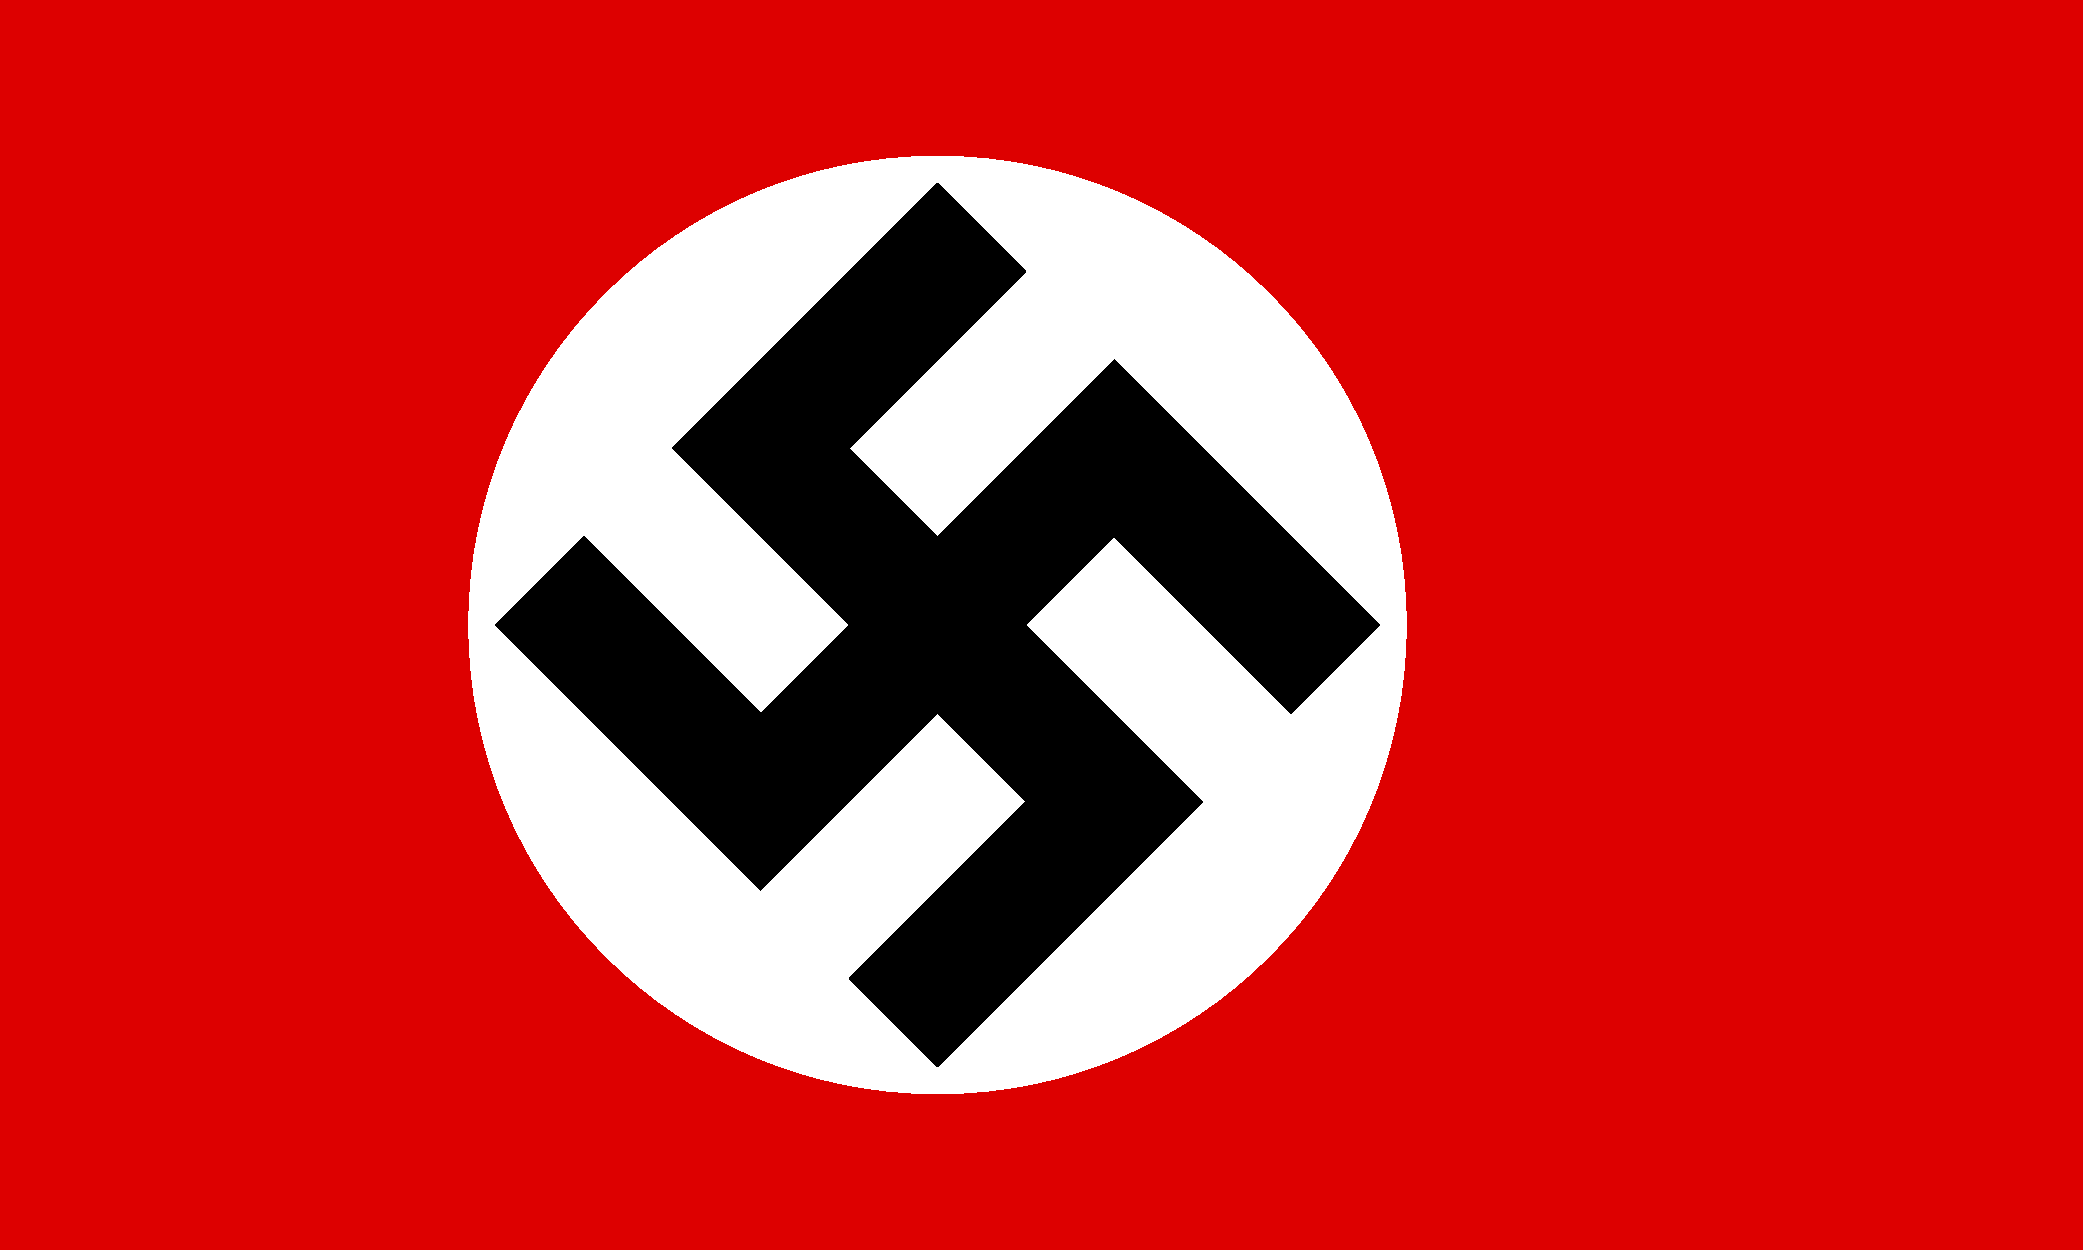
\includegraphics[width=1.0\linewidth]{Annexes/friseChronologique/img/Flag_of_Germany_281935E28093194529.pdf}
            \end{figure}
        \end{minipage}
    &
        \begin{minipage}{.65\textwidth}
            \textbf{1942} - \textbf{Le Messerschmitt Me 262, premier chasseur à réaction}
            
            Premier chasseur à réaction de l'Histoire, sa mise au point fut cependant longue et son entrée en service dans la Luftwaffe (armée de l'air allemande) en avril 1944 (donc à la fin de la guerre) impliquera que cet avion aura un rôle mineur dans le second conflit mondial.
            \begin{figure}[H]
                \legende{Un Messerschmitt Me 262}{frise:Messerschmitt_Me_262A_at_the_National_Museum_of_the_USAF.jpg}
            \end{figure}
        \end{minipage}
    &
        \begin{minipage}{.275\textwidth}
            \begin{figure}[H]
                \centering
                \includegraphics[width=1.0\linewidth]{Annexes/friseChronologique/img/Messerschmitt_Me_262A_at_the_National_Museum_of_the_USAF.jpg}
            \end{figure}
        \end{minipage}
    \end{tabular}
\end{table}
\begin{table}[H]
    \centering
    \begin{tabular}{c l c}
        \begin{minipage}{.075\textwidth}
            \begin{figure}[H]
                \centering
                \includegraphics[width=1.0\linewidth]{Annexes/friseChronologique/img/Flag_of_the_United_States_28DDD-F-416E_specifications29.pdf}
            \end{figure}
        \end{minipage}
    &
        \begin{minipage}{.65\textwidth}
            \textbf{1943} - \textbf{Jacqueline Cochran crée le Women Airforce Service Pilots}
            
            
        \end{minipage}
    &
        \begin{minipage}{.275\textwidth}
            \begin{figure}[H]
                \centering
                \includegraphics[width=1.0\linewidth]{Annexes/friseChronologique/vide.pdf}
            \end{figure}
        \end{minipage}
    \end{tabular}
\end{table}
\section{L'age d'or de la réaction et la guerre froide}

\begin{table}[H]
    \centering
    \begin{tabular}{c l c}
        \begin{minipage}{.075\textwidth}
            \begin{figure}[H]
                \centering
                \includegraphics[width=1.0\linewidth]{Annexes/friseChronologique/img/Flag_of_the_United_States_28DDD-F-416E_specifications29.pdf}
            \end{figure}
        \end{minipage}
    &
        \begin{minipage}{.65\textwidth}
            \textbf{1947} - \textbf{Chuck Yeager franchit le mur du son}
            
            Chuck Yeager devient le premier humain à franchir le mur du son, à bord du Bell X1.
            \begin{figure}[H]
                \legende{L'avion fusée Bell X1}{frise:Bell_X-1_46-062_28in_flight29.jpg}
            \end{figure}
        \end{minipage}
    &
        \begin{minipage}{.275\textwidth}
            \begin{figure}[H]
                \centering
                \includegraphics[width=1.0\linewidth]{Annexes/friseChronologique/img/Bell_X-1_46-062_28in_flight29.jpg}
            \end{figure}
        \end{minipage}
    \end{tabular}
\end{table}
\begin{table}[H]
    \centering
    \begin{tabular}{c l c}
        \begin{minipage}{.075\textwidth}
            \begin{figure}[H]
                \centering
                \includegraphics[width=1.0\linewidth]{Annexes/friseChronologique/img/Flag_of_France.pdf}
            \end{figure}
        \end{minipage}
    &
        \begin{minipage}{.65\textwidth}
            \textbf{1953} - \textbf{Création de la patrouille de France}
            
            
            \begin{figure}[H]
                \legende{Photo récente de la Patrouille de France, sur AlphaJet}{frise:Alphajet_5_en_passage_au_meeting_d27Orange_2019.jpg}
            \end{figure}
        \end{minipage}
    &
        \begin{minipage}{.275\textwidth}
            \begin{figure}[H]
                \centering
                \includegraphics[width=1.0\linewidth]{Annexes/friseChronologique/img/Alphajet_5_en_passage_au_meeting_d27Orange_2019.jpg}
            \end{figure}
        \end{minipage}
    \end{tabular}
\end{table}
\begin{table}[H]
    \centering
    \begin{tabular}{c l c}
        \begin{minipage}{.075\textwidth}
            \begin{figure}[H]
                \centering
                \includegraphics[width=1.0\linewidth]{Annexes/friseChronologique/img/Flag_of_France.pdf}
            \end{figure}
        \end{minipage}
    &
        \begin{minipage}{.65\textwidth}
            \textbf{1953} - \textbf{Jacqueline Auriol, première femme européenne à franchir le mur du son}
            
            
            \begin{figure}[H]
                \legende{Jacqueline Auriol en 1947}{frise:Auriol_Harcourt_1947_2.jpg}
            \end{figure}
        \end{minipage}
    &
        \begin{minipage}{.275\textwidth}
            \begin{figure}[H]
                \centering
                \includegraphics[width=1.0\linewidth]{Annexes/friseChronologique/img/Auriol_Harcourt_1947_2.jpg}
            \end{figure}
        \end{minipage}
    \end{tabular}
\end{table}
\begin{table}[H]
    \centering
    \begin{tabular}{c l c}
        \begin{minipage}{.075\textwidth}
            \begin{figure}[H]
                \centering
                \includegraphics[width=1.0\linewidth]{Annexes/friseChronologique/img/Flag_of_the_Soviet_Union.pdf}
            \end{figure}
        \end{minipage}
    &
        \begin{minipage}{.65\textwidth}
            \textbf{1957} - \textbf{Spoutnik 1, premier satellite artificiel}
            
            Lancé par l'URSS
            \begin{figure}[H]
                \legende{Une réplique de Spoutnik 1}{frise:Sputnik_asm.jpg}
            \end{figure}
        \end{minipage}
    &
        \begin{minipage}{.275\textwidth}
            \begin{figure}[H]
                \centering
                \includegraphics[width=1.0\linewidth]{Annexes/friseChronologique/img/Sputnik_asm.jpg}
            \end{figure}
        \end{minipage}
    \end{tabular}
\end{table}
\begin{table}[H]
    \centering
    \begin{tabular}{c l c}
        \begin{minipage}{.075\textwidth}
            \begin{figure}[H]
                \centering
                \includegraphics[width=1.0\linewidth]{Annexes/friseChronologique/img/Flag_of_the_Soviet_Union.pdf}
            \end{figure}
        \end{minipage}
    &
        \begin{minipage}{.65\textwidth}
            \textbf{1961} - \textbf{Youri Gagarine, premier humain dans l'espace}
            
            Le soviétique Youri Gagarine devient le premier cosmonaute lors de la mission Vostok 1. Il effectue 1 orbite autour de la Terre en 1h48.
            \begin{figure}[H]
                \legende{Photo de Youri Gagarine}{frise:Yuri_Gagarin_28196129.jpg}
            \end{figure}
        \end{minipage}
    &
        \begin{minipage}{.275\textwidth}
            \begin{figure}[H]
                \centering
                \includegraphics[width=1.0\linewidth]{Annexes/friseChronologique/img/Yuri_Gagarin_28196129.jpg}
            \end{figure}
        \end{minipage}
    \end{tabular}
\end{table}
\begin{table}[H]
    \centering
    \begin{tabular}{c l c}
        \begin{minipage}{.075\textwidth}
            \begin{figure}[H]
                \centering
                \includegraphics[width=1.0\linewidth]{Annexes/friseChronologique/img/Flag_of_the_Soviet_Union.pdf}
            \end{figure}
        \end{minipage}
    &
        \begin{minipage}{.65\textwidth}
            \textbf{1963} - \textbf{Valentina Terechkova, première femme dans l'espace}
            
            La soviétique Valentina Terechkova devient la première femme s'être rendue dans l'espace, lors de la mission Vostok 6
            \begin{figure}[H]
                \legende{Les cosmonautes Valentina Terechkova avec Valeri Bykovski après le retour sur Terre en juin 1963.}{frise:RIAN_archive_15491_Valery_Bykovsky_and_Valentina_Tereshkova.jpg}
            \end{figure}
        \end{minipage}
    &
        \begin{minipage}{.275\textwidth}
            \begin{figure}[H]
                \centering
                \includegraphics[width=1.0\linewidth]{Annexes/friseChronologique/img/RIAN_archive_15491_Valery_Bykovsky_and_Valentina_Tereshkova.jpg}
            \end{figure}
        \end{minipage}
    \end{tabular}
\end{table}
\begin{table}[H]
    \centering
    \begin{tabular}{c l c}
        \begin{minipage}{.075\textwidth}
            \begin{figure}[H]
                \centering
                \includegraphics[width=1.0\linewidth]{Annexes/friseChronologique/img/Flag_of_France.pdf}
            \end{figure}
        \end{minipage}
    &
        \begin{minipage}{.65\textwidth}
            \textbf{1965} - \textbf{Asterix, premier satellite français}
            
            La France lance en 1965 son premier satellite : Asterix. Il est lancé par une fusée Diament-A, également de conception française.
Si la France n'est que la sixième nation à lancer une satellite, elle est la troisième à le faire avec sa propre fusée, aprés les soviétiques (1957, Spoutnik 1) et les Etats-Unis (1958, Explorer 1)
            \begin{figure}[H]
                \legende{Satellite A1 Astérix, premier satellite francais (1965) modèle d'essais }{frise:Asterix_Musee_du_Bourget_P1020341.JPG}
            \end{figure}
        \end{minipage}
    &
        \begin{minipage}{.275\textwidth}
            \begin{figure}[H]
                \centering
                \includegraphics[width=1.0\linewidth]{Annexes/friseChronologique/img/Asterix_Musee_du_Bourget_P1020341.JPG}
            \end{figure}
        \end{minipage}
    \end{tabular}
\end{table}
\begin{table}[H]
    \centering
    \begin{tabular}{c l c}
        \begin{minipage}{.075\textwidth}
            \begin{figure}[H]
                \centering
                \includegraphics[width=1.0\linewidth]{Annexes/friseChronologique/img/Flag_of_the_United_States_28DDD-F-416E_specifications29.pdf}
            \end{figure}
        \end{minipage}
    &
        \begin{minipage}{.65\textwidth}
            \textbf{1969} - \textbf{Pemier vol du Boeing 747}
            
            Le "Jumbo Jet" Boeing 747 effectue son premier vol. Cet avion gros porteur ouvre l'ère du transport aérien de masse.
            \begin{figure}[H]
                \legende{Boeing 747-200 en 1980}{frise:B-747_Iberia.jpg}
            \end{figure}
        \end{minipage}
    &
        \begin{minipage}{.275\textwidth}
            \begin{figure}[H]
                \centering
                \includegraphics[width=1.0\linewidth]{Annexes/friseChronologique/img/B-747_Iberia.jpg}
            \end{figure}
        \end{minipage}
    \end{tabular}
\end{table}
\begin{table}[H]
    \centering
    \begin{tabular}{c l c}
        \begin{minipage}{.075\textwidth}
            \begin{figure}[H]
                \centering
                \includegraphics[width=1.0\linewidth]{Annexes/friseChronologique/img/Flag_of_France.pdf}
            \end{figure}
        \end{minipage}
    &
        \begin{minipage}{.65\textwidth}
            \textbf{1969} - \textbf{Premier vol du Concorde}
            
            Le Concorde effectue son premier vol avec le pilote d'essai André Turcat aux commandes.

Le 1er octobre 1969, le Concorde franchit pour la première fois le mur du son avec Jean Pinet en tant que commande de bord.

Concorde demeure à ce jour le seul avion supersonique qui aura eu une carrière commerciale notable puisque sa carrière durera de 1976, date de son premier vol commercial, à 2003 (son concurrent soviétique, le Tupolev Tu-144 ne sera exploité commercialement que quelques mois et environ 50 vols à la fin de les années 1970)
            \begin{figure}[H]
                \legende{Concorde British Airways}{frise:British_Airways_Concorde_G-BOAC_03.jpg}
            \end{figure}
        \end{minipage}
    &
        \begin{minipage}{.275\textwidth}
            \begin{figure}[H]
                \centering
                \includegraphics[width=1.0\linewidth]{Annexes/friseChronologique/img/British_Airways_Concorde_G-BOAC_03.jpg}
            \end{figure}
        \end{minipage}
    \end{tabular}
\end{table}
\begin{table}[H]
    \centering
    \begin{tabular}{c l c}
        \begin{minipage}{.075\textwidth}
            \begin{figure}[H]
                \centering
                \includegraphics[width=1.0\linewidth]{Annexes/friseChronologique/img/Flag_of_the_United_States_28DDD-F-416E_specifications29.pdf}
            \end{figure}
        \end{minipage}
    &
        \begin{minipage}{.65\textwidth}
            \textbf{1969} - \textbf{L'Homme est sur la Lune}
            
            "Un petit pas pour l'Homme, un bond de géant pour l'Humanité". Neil Armstrong est le premier humain à fouler le sol lunaire durant la mission Apollo 11. Leur vaisseau lunaire, propulsé par une fusée Saturne 5, lui permettra, ainsi qu'a ses collègues de mission, Buzz Aldrin et Michael Collins (ce dernier étant resté en orbite autour de la Lune durant la mission), de rentrer dans l'Histoire.
            \begin{figure}[H]
                \legende{Photo de Buzz Aldrin sur la Lune}{frise:A_Man_on_the_Moon2C_AS11-40-5903.jpg}
            \end{figure}
        \end{minipage}
    &
        \begin{minipage}{.275\textwidth}
            \begin{figure}[H]
                \centering
                \includegraphics[width=1.0\linewidth]{Annexes/friseChronologique/img/A_Man_on_the_Moon2C_AS11-40-5903.jpg}
            \end{figure}
        \end{minipage}
    \end{tabular}
\end{table}
\section{L'ère de l'efficience}
Suite au premier choc pétrolier de 1973, l'aéronautique entre dans une phase ou la dimension énégétique est prise en compte dans la conception des aéronefs
\begin{table}[H]
    \centering
    \begin{tabular}{c l c}
        \begin{minipage}{.075\textwidth}
            \begin{figure}[H]
                \centering
                \includegraphics[width=1.0\linewidth]{Annexes/friseChronologique/img/Flag_of_the_United_States_28DDD-F-416E_specifications29.pdf}
            \end{figure}
        \end{minipage}
    &
        \begin{minipage}{.65\textwidth}
            \textbf{1981} - \textbf{Premier vol de la navette spatiale américaine}
            
            La navette Columbia, affectée à la mission STS-1, effectue le vol inaugural des navette spatiales américaines
            \begin{figure}[H]
                \legende{Décollage de Columbia pour la mission STS-1}{frise:Space_Shuttle_Columbia_launching.jpg}
            \end{figure}
        \end{minipage}
    &
        \begin{minipage}{.275\textwidth}
            \begin{figure}[H]
                \centering
                \includegraphics[width=1.0\linewidth]{Annexes/friseChronologique/img/Space_Shuttle_Columbia_launching.jpg}
            \end{figure}
        \end{minipage}
    \end{tabular}
\end{table}
\begin{table}[H]
    \centering
    \begin{tabular}{c l c}
        \begin{minipage}{.075\textwidth}
            \begin{figure}[H]
                \centering
                \includegraphics[width=1.0\linewidth]{Annexes/friseChronologique/img/Flag_of_France.pdf}
            \end{figure}
        \end{minipage}
    &
        \begin{minipage}{.65\textwidth}
            \textbf{1982} - \textbf{Jean-Loup Chrétien, premier astronaute français}
            
            Jean-Loup Chrétien devient le premier astronaute européen de l'ouest, à l'occasion d'une mission dans la station soviétique Saliout 7.

Il effectuera un second séjour dans la station Mir en 1988.

Il cumule environ 44 jours dans l'espace.
            \begin{figure}[H]
                \legende{Portrait officiel NASA de Jean-Loup Chrétien}{frise:Jean-Loup_Jacques_Marie_ChrC3A9tien2C_French_Spationaut_28NASA29.jpg}
            \end{figure}
        \end{minipage}
    &
        \begin{minipage}{.275\textwidth}
            \begin{figure}[H]
                \centering
                \includegraphics[width=1.0\linewidth]{Annexes/friseChronologique/img/Jean-Loup_Jacques_Marie_ChrC3A9tien2C_French_Spationaut_28NASA29.jpg}
            \end{figure}
        \end{minipage}
    \end{tabular}
\end{table}
\begin{table}[H]
    \centering
    \begin{tabular}{c l c}
        \begin{minipage}{.075\textwidth}
            \begin{figure}[H]
                \centering
                \includegraphics[width=1.0\linewidth]{Annexes/friseChronologique/img/Flag_of_France.pdf}
            \end{figure}
        \end{minipage}
    &
        \begin{minipage}{.65\textwidth}
            \textbf{1987} - \textbf{Premier vol de l'Airbus A320}
            
            
        \end{minipage}
    &
        \begin{minipage}{.275\textwidth}
            \begin{figure}[H]
                \centering
                \includegraphics[width=1.0\linewidth]{Annexes/friseChronologique/vide.pdf}
            \end{figure}
        \end{minipage}
    \end{tabular}
\end{table}
\begin{table}[H]
    \centering
    \begin{tabular}{c l c}
        \begin{minipage}{.075\textwidth}
            \begin{figure}[H]
                \centering
                \includegraphics[width=1.0\linewidth]{Annexes/friseChronologique/img/Flag_of_France.pdf}
            \end{figure}
        \end{minipage}
    &
        \begin{minipage}{.65\textwidth}
            \textbf{1996} - \textbf{Claudie Haigneré, première spationaute française}
            
            14 ans après le premier français dans l'espace, Claudie Haigneré devient la première française (et premiere femme Européenne non soviétique) dans l'espace, avec un séjour dans la station russe Mir.

En 2001, elle effectue un second séjour dans l'espace, à bord de la station spatiale internationale.

Elle cumule ainsi environ 25 jours dans l'espace.
            \begin{figure}[H]
                \legende{Claudie Haigneré (à droite) dans l'ISS, en 2001}{frise:ISS-03_Soyuz_TM-33_Taxi_crewmembers_in_the_Zvezda_Service_Module.jpg}
            \end{figure}
        \end{minipage}
    &
        \begin{minipage}{.275\textwidth}
            \begin{figure}[H]
                \centering
                \includegraphics[width=1.0\linewidth]{Annexes/friseChronologique/img/ISS-03_Soyuz_TM-33_Taxi_crewmembers_in_the_Zvezda_Service_Module.jpg}
            \end{figure}
        \end{minipage}
    \end{tabular}
\end{table}
\begin{table}[H]
    \centering
    \begin{tabular}{c l c}
        \begin{minipage}{.075\textwidth}
            \begin{figure}[H]
                \centering
                \includegraphics[width=1.0\linewidth]{Annexes/friseChronologique/img/Flag_of_France.pdf}
            \end{figure}
        \end{minipage}
    &
        \begin{minipage}{.65\textwidth}
            \textbf{1999} - \textbf{Caroline Aigle, première pilote de chasse française}
            
            Le 28 mai 1999, Caroline Aigle est brevetée pilote de chasse. Elle devient la première femme francaise pilote de chasse. Elle sera notamment affectéé sur Mirage 2000.
            \begin{figure}[H]
                \legende{Caroline Aigle (1974-2007), aviatrice, pilote de chasse.}{frise:Caroline_Aigle_portrait.jpg}
            \end{figure}
        \end{minipage}
    &
        \begin{minipage}{.275\textwidth}
            \begin{figure}[H]
                \centering
                \includegraphics[width=1.0\linewidth]{Annexes/friseChronologique/img/Caroline_Aigle_portrait.jpg}
            \end{figure}
        \end{minipage}
    \end{tabular}
\end{table}
\begin{table}[H]
    \centering
    \begin{tabular}{c l c}
        \begin{minipage}{.075\textwidth}
            \begin{figure}[H]
                \centering
                \includegraphics[width=1.0\linewidth]{Annexes/friseChronologique/img/Flag_of_Europe.pdf}
            \end{figure}
        \end{minipage}
    &
        \begin{minipage}{.65\textwidth}
            \textbf{2005} - \textbf{Premier vol de l'A380}
            
            L'Airbus A380, plus gros avion de transport commercial du monde, effectue son premier vol en 2005.

Cet avion est certifié pour emporter jusqu'à 853 passagers.
            \begin{figure}[H]
                \legende{A380 en vol}{frise:A6-EDY_A380_Emirates_31_jan_2013_jfk_28844226936429_28cropped29.jpg}
            \end{figure}
        \end{minipage}
    &
        \begin{minipage}{.275\textwidth}
            \begin{figure}[H]
                \centering
                \includegraphics[width=1.0\linewidth]{Annexes/friseChronologique/img/A6-EDY_A380_Emirates_31_jan_2013_jfk_28844226936429_28cropped29.jpg}
            \end{figure}
        \end{minipage}
    \end{tabular}
\end{table}
\begin{table}[H]
    \centering
    \begin{tabular}{c l c}
        \begin{minipage}{.075\textwidth}
            \begin{figure}[H]
                \centering
                \includegraphics[width=1.0\linewidth]{Annexes/friseChronologique/img/Flag_of_Austria.pdf}
            \end{figure}
        \end{minipage}
    &
        \begin{minipage}{.65\textwidth}
            \textbf{2012} - \textbf{Felix Baumgartner franchit le mur du son en chute libre}
            
            Après s'être lancé d'un ballon à gaz à près de 40 km d'altitude, le parachutiste Felix Baumgartner réalise un saut durant lequel il deviendra le premier à franchir le mur du son en chute libre 
        \end{minipage}
    &
        \begin{minipage}{.275\textwidth}
            \begin{figure}[H]
                \centering
                \includegraphics[width=1.0\linewidth]{Annexes/friseChronologique/vide.pdf}
            \end{figure}
        \end{minipage}
    \end{tabular}
\end{table}
\begin{table}[H]
    \centering
    \begin{tabular}{c l c}
        \begin{minipage}{.075\textwidth}
            \begin{figure}[H]
                \centering
                \includegraphics[width=1.0\linewidth]{Annexes/friseChronologique/img/Flag_of_Switzerland_28Pantone29.pdf}
            \end{figure}
        \end{minipage}
    &
        \begin{minipage}{.65\textwidth}
            \textbf{2015} - \textbf{Solar Impulse : tour du monde}
            
            Solar Impulse devient le premier avon à réaliser un tour du monde 100% éléctrique, alimenté notamment par ses panneaux solaires
            \begin{figure}[H]
                \legende{Solar Impulse SI2 à Payerne le 13 novembre 2014}{frise:Solar_Impulse_SI2_pilote_Bertrand_Piccard_Payerne_November_2014.jpg}
            \end{figure}
        \end{minipage}
    &
        \begin{minipage}{.275\textwidth}
            \begin{figure}[H]
                \centering
                \includegraphics[width=1.0\linewidth]{Annexes/friseChronologique/img/Solar_Impulse_SI2_pilote_Bertrand_Piccard_Payerne_November_2014.jpg}
            \end{figure}
        \end{minipage}
    \end{tabular}
\end{table}
\begin{table}[H]
    \centering
    \begin{tabular}{c l c}
        \begin{minipage}{.075\textwidth}
            \begin{figure}[H]
                \centering
                \includegraphics[width=1.0\linewidth]{Annexes/friseChronologique/img/Flag_of_Europe.pdf}
            \end{figure}
        \end{minipage}
    &
        \begin{minipage}{.65\textwidth}
            \textbf{2024} - \textbf{Premier vol d'Ariane 6}
            
            La fusée Ariane 6 effectue son vol inaugural. Le premier vol commercial de ce nouveau lancer de l'agence spatiale européenne aura lieu un peu plus tard, en mars 2025
            \begin{figure}[H]
                \legende{Ariane 6 sur son pas de tir}{frise:Ariane_6_on_pad.jpg}
            \end{figure}
        \end{minipage}
    &
        \begin{minipage}{.275\textwidth}
            \begin{figure}[H]
                \centering
                \includegraphics[width=1.0\linewidth]{Annexes/friseChronologique/img/Ariane_6_on_pad.jpg}
            \end{figure}
        \end{minipage}
    \end{tabular}
\end{table}
